\documentclass[student]{ITRslides}

\addbibresource{ref.bib}
\graphicspath{{pics/}{logos/}}

\title{Control of a multi-robot cooperative team guided by a human operator}
\presenter{M. Angerer}

\supervisor{S. Musi\'c}
\typeofpres{Intermediate Presentation Master Thesis}



%%%%%%%%%%%%%%%%%%%%%%%%%%%%%%%%%%%%%%%%%%%%%%%%%%%%%%%%%%%%%%%%%%%%%%%%%%%%%%%%

\begin{document}


\begin{frame}
    \titlepage
\end{frame}

%\begin{frame}
%	\frametitle{Overview}
%    \tableofcontents%[hideallsubsections]%[pausesections]
%\end{frame}

\section{Introduction}

\begin{frame}
	\frametitle{Why use cooperative manipulation with human guidance?}
		\begin{columns}
		\column{0.55\linewidth}
			\begin{figure}[htb]
			\centering
			%\psfrag{q1}[Bl][Bl]{\small $\alpha$}
			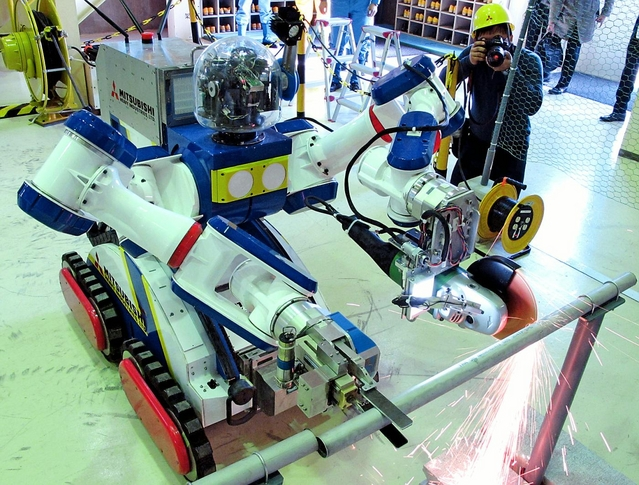
\includegraphics[width=0.98\textwidth]{mhi-meister45.jpg}
			\caption{Demonstration of MHI MEISTeR at 						Fukushima Daiichi 					Nuclear 						Power Station\cite{}}
			\end{figure} 
		\column{0.55\linewidth}
		Human reasoning
		\begin{itemize}
			\item Foresight and adaptiveness to incidents
			\item superior planning capabilities
		\end{itemize}
		Enhanced flexibility of multiple robots
			\begin{itemize}
				\item transportation of large/heavy objects
	\item assembly of multiple parts 
	\item coordinated use of tools
			\end{itemize}
			\end{columns}
\end{frame}

\begin{frame}
	\frametitle{Problem Formulation}

	\begin{itemize}
		\item Precise and stable control during free-motion/contact transition
		\item Enhance versatility by performing friction grasps
		\item (Intuitive) high-level human supervisory control
		\item Local formation requirements controlled by robots
		\item Assistance of the operator with suitable feedback
		\item Preservation of stability over delayed communication (?, very vulnerable point) 
	\end{itemize}

\end{frame}

\begin{frame}
	\frametitle{Related Work: Impedance Control}
	\begin{itemize}
		\item Formation control of robot team \cite{Sieber_15,Wimboeck_06}
		\begin{itemize}
			\item object not part of control loop
			%\item no knowledge of object required
		\end{itemize}
		\item Intrinsically Passive Control \cite{Stramigioli_01, Wimboeck_08}
		\begin{itemize}
			\item virtual object simulation
			%\item knowledge of object shape and dynamics required
		\end{itemize}
		\item Internal impedance control + object dynamics' feed-forward \cite{DePascali_15}
				\begin{itemize}
			\item object tracking required
			%\item knowledge of object shape and dynamics required
		\end{itemize}
		\item Internal and external impedance control \cite{Caccavale_01,Caccavale_08}
			\begin{itemize}
			%\item object tracking required
			%\item knowledge of object shape and dynamics required
			\item Force/Torque sensors at the manipulators required
			\end{itemize}
	\end{itemize}
\end{frame}

\begin{frame}
	\frametitle{Related Work: Human in the loop}
	\begin{itemize}
		\item Bilateral tele-manipulation  \cite{Lee_05}
		\begin{itemize}
			\item Single master, constrained system as slave
			\item Local control of interaction dynamics
			\item Force feedback
		\end{itemize}
		\item Formation-based shared control \cite{Sieber_15, Scheggi_14}
		\begin{itemize}
			\item Single leader, multiple followers
			\item Robots preserve formation autonomously
			\item Tactile feedback
		\end{itemize}
		\item Gesture Control \cite{Gioioso_2014}
		\begin{itemize}
			\item Hand motion controls constrained system
			\item Hand pose controls grasping process
			%\item only visual feedback
		\end{itemize}
		\end{itemize}
\end{frame}

\section{Approach}

\begin{frame}
	\frametitle{Energy consistent modelling and control}
	\begin{itemize}
		\item controlled robots are passive
		\item operator and environment can supply energy
		\item effort-flow pair: force and velocity
		\end{itemize}
\begin{itemize}%[leftmargin=0em]
  \renewcommand{\labelitemi}{$\Rightarrow$}
\item enhanced human perception through control of a meaningful quantity and appropriate feedback
\item stability over a wide class of environments
			\end{itemize}
		\begin{quote}
		If a controlled robot is not passive there is always a passive environment that destabilizes the interconnected system \cite{Stramigioli_15}
		\end{quote}


\end{frame}
\begin{frame}
	\frametitle{Interconnection of energy-discrete elements}
	\begin{itemize}
		\item mechanical elements
			\begin{itemize}
			\item spring
			\item mass
			\item damper
			\end{itemize}
		\item conservative elements
			\begin{itemize}
			\item transformer
			\item gyrator
			\end{itemize}
		\item interconnection through power ports
		\[ \mathcal{P} = \mathcal{V} \times \mathcal{V}^* \]
		\end{itemize}



\end{frame}

%\begin{frame}
%	\frametitle{Intrinsically Passive Control (IPC)}
%	\begin{columns}
%		\column{0.4\linewidth}
%			
%	
%		\begin{itemize}
%			\item High-level Supervisor and low-level IPC
%			\item IPC + robot: passive
%			\item Power provided by Supervisor
%			\item Environment assumed passive
%		\end{itemize}
%
%		
%		\column{0.58\linewidth}
%             \begin{figure}[htb]
%			\centering
%			%\psfrag{q1}[Bl][Bl]{\small $\alpha$}
%			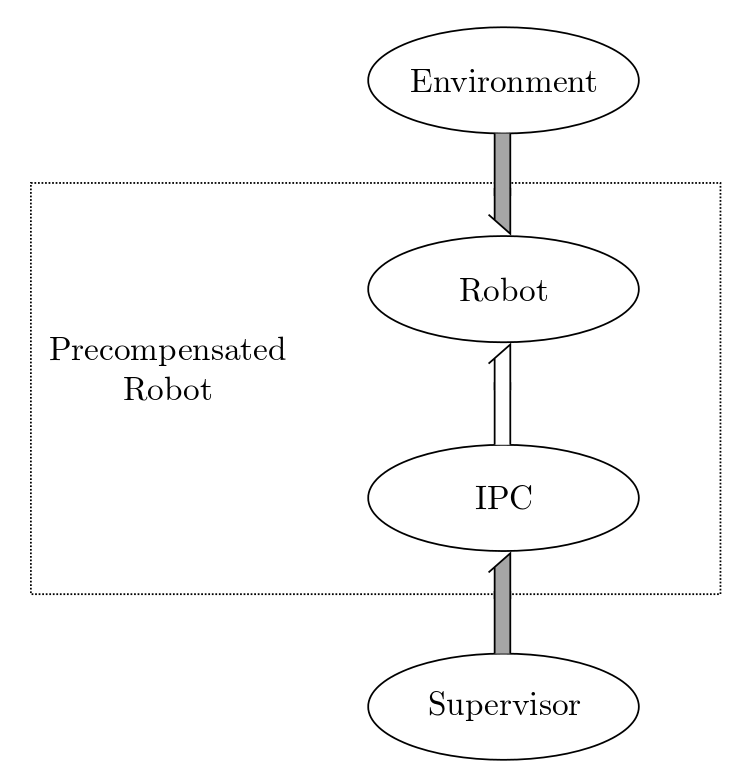
\includegraphics[width=0.9\textwidth]{IPCoverview.png}
%			\caption{Overview of the IPC architecture 								\cite{Stramigioli_01}}
%			\end{figure}
%		
%			
%		\end{columns}
%\end{frame}

\begin{frame}
	\frametitle{Structure of the IPC}
\begin{columns}
		\column{0.5\linewidth}
			
	
		\begin{itemize}
			\item Spring-mass-damper system
			\item Simulated virtual object
			\item Manipulators modelled by inertias
			\item Potential (inertia) and kinetic (springs) energy
			\item Energy dissipation in damper: passivity
		\end{itemize}

		
		\column{0.5\linewidth}
             \begin{figure}[htb]
			\centering
			%\psfrag{q1}[Bl][Bl]{\small $\alpha$}
			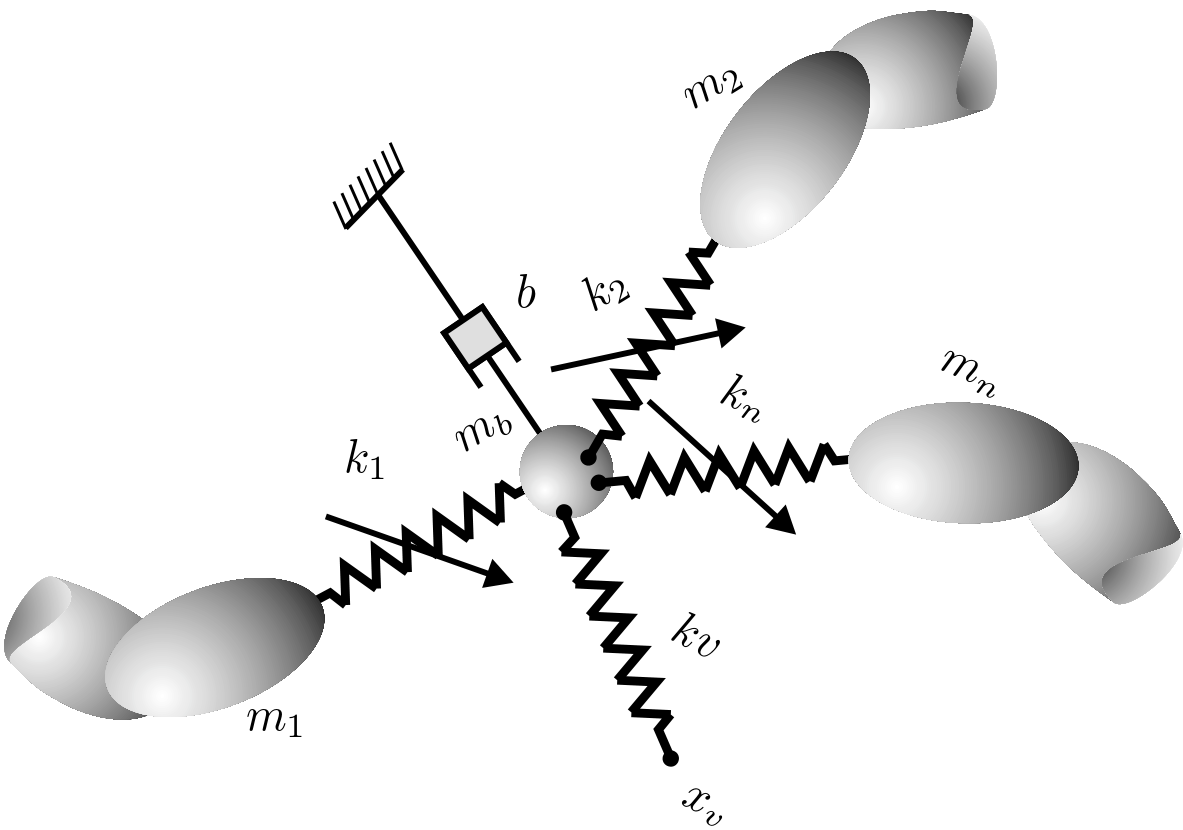
\includegraphics[width=0.98\textwidth]{IPCsprings.png}
			\caption{Mass-spring-damper structure of the IPC 						\cite{Stramigioli_01}}
			\end{figure}
		
			
		\end{columns}
\end{frame}

\begin{frame}
	\frametitle{Grasping an object}
\begin{columns}
		\column{0.4\linewidth}
			
	
		\begin{itemize}
			\item Variable rest-length springs
			\item Rest-length: virtual object size
			\item Distinct power port
		\end{itemize}

		
		\column{0.62\linewidth}
             \begin{figure}[htb]
			\centering
			%\psfrag{q1}[Bl][Bl]{\small $\alpha$}
			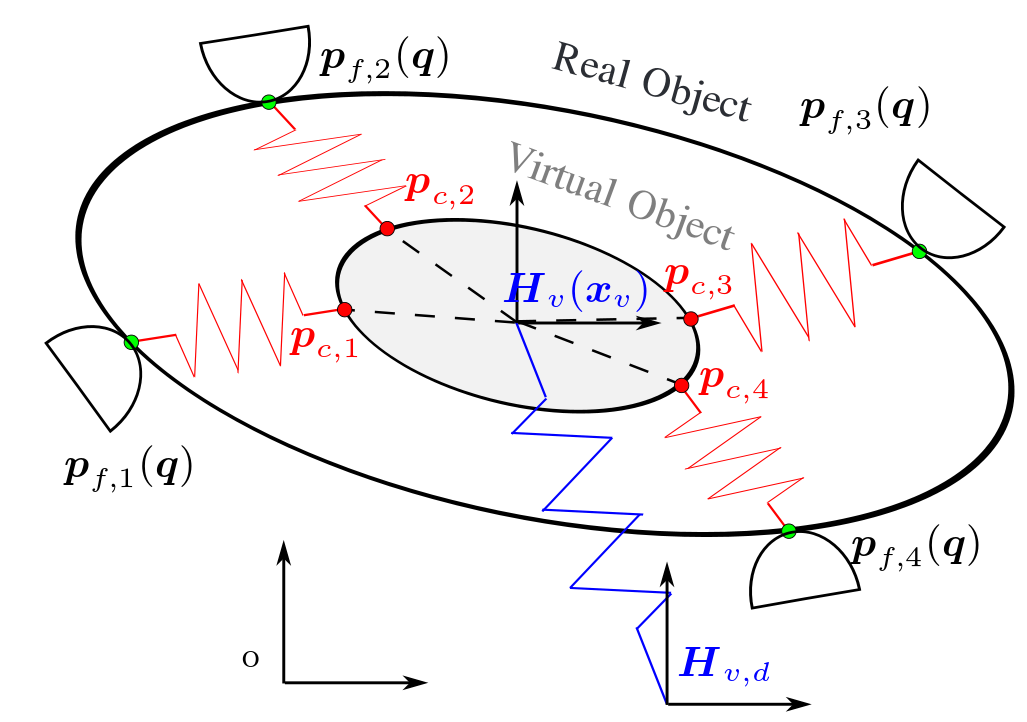
\includegraphics[width=0.98\textwidth]{IPCobjects.png}
			\caption{Virtual and real object \cite{Wimboeck_08}}
			\end{figure}
		
			
		\end{columns}
\end{frame}

%\begin{frame}
%	\frametitle{The Supervisor}
%	\begin{itemize}
%			\item Two power ports per IPC-robot-system
%			\item Human operator takes role of Supervisor
%			\item Connected via delayed communication line
%		\end{itemize}
%\end{frame}

%\begin{frame}
%	\frametitle{Tele-operation}
%	\begin{itemize}
%			\item Preserving passivity
%			\item Scattering or Wave variables
%		\end{itemize}
%\end{frame}

\section{Results}
\begin{frame}
	\frametitle{Grasping force optimization for friction contacts}
	\begin{columns}
	\column{0.6\textwidth}
	\begin{itemize}
	\item required contact normal force is dependent on tangential forces
	\item high tangential forces arise during acceleration
	\item other requirements: safety margin, maximum grasping force $\Rightarrow$ cost function
	\item linear matrix inequality (LMI) problem
	\end{itemize}
	\column{0.5\textwidth}

\begin{figure}[htb]
			\centering
			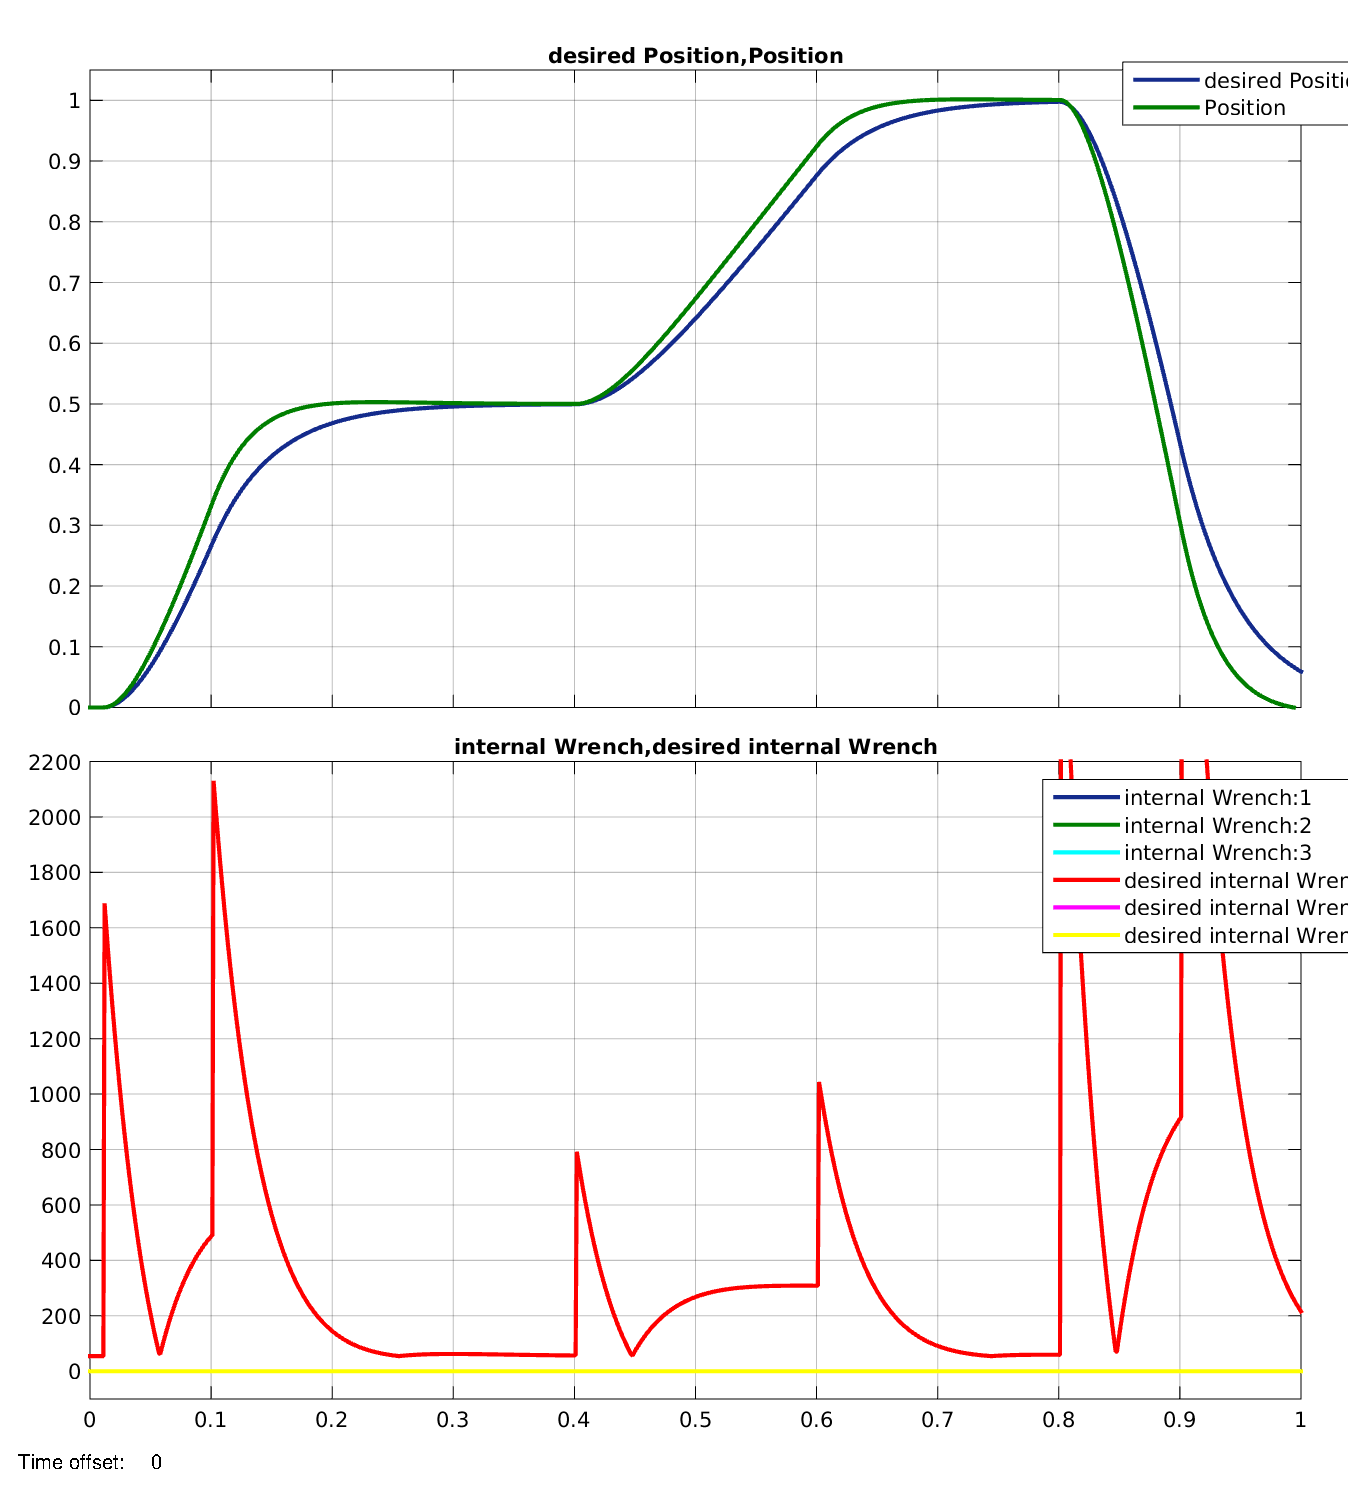
\includegraphics[width=0.9\textwidth]{Hanposforce.eps}
			\caption{Position, Internal wrench}
\end{figure}
\end{columns}
\end{frame}
\begin{frame}
	\frametitle{Comparison of Grasp Controllers 1}
Impedance-based reference trajectory generation \cite{Caccavale_01}
 \begin{figure}[htb]
			\centering
			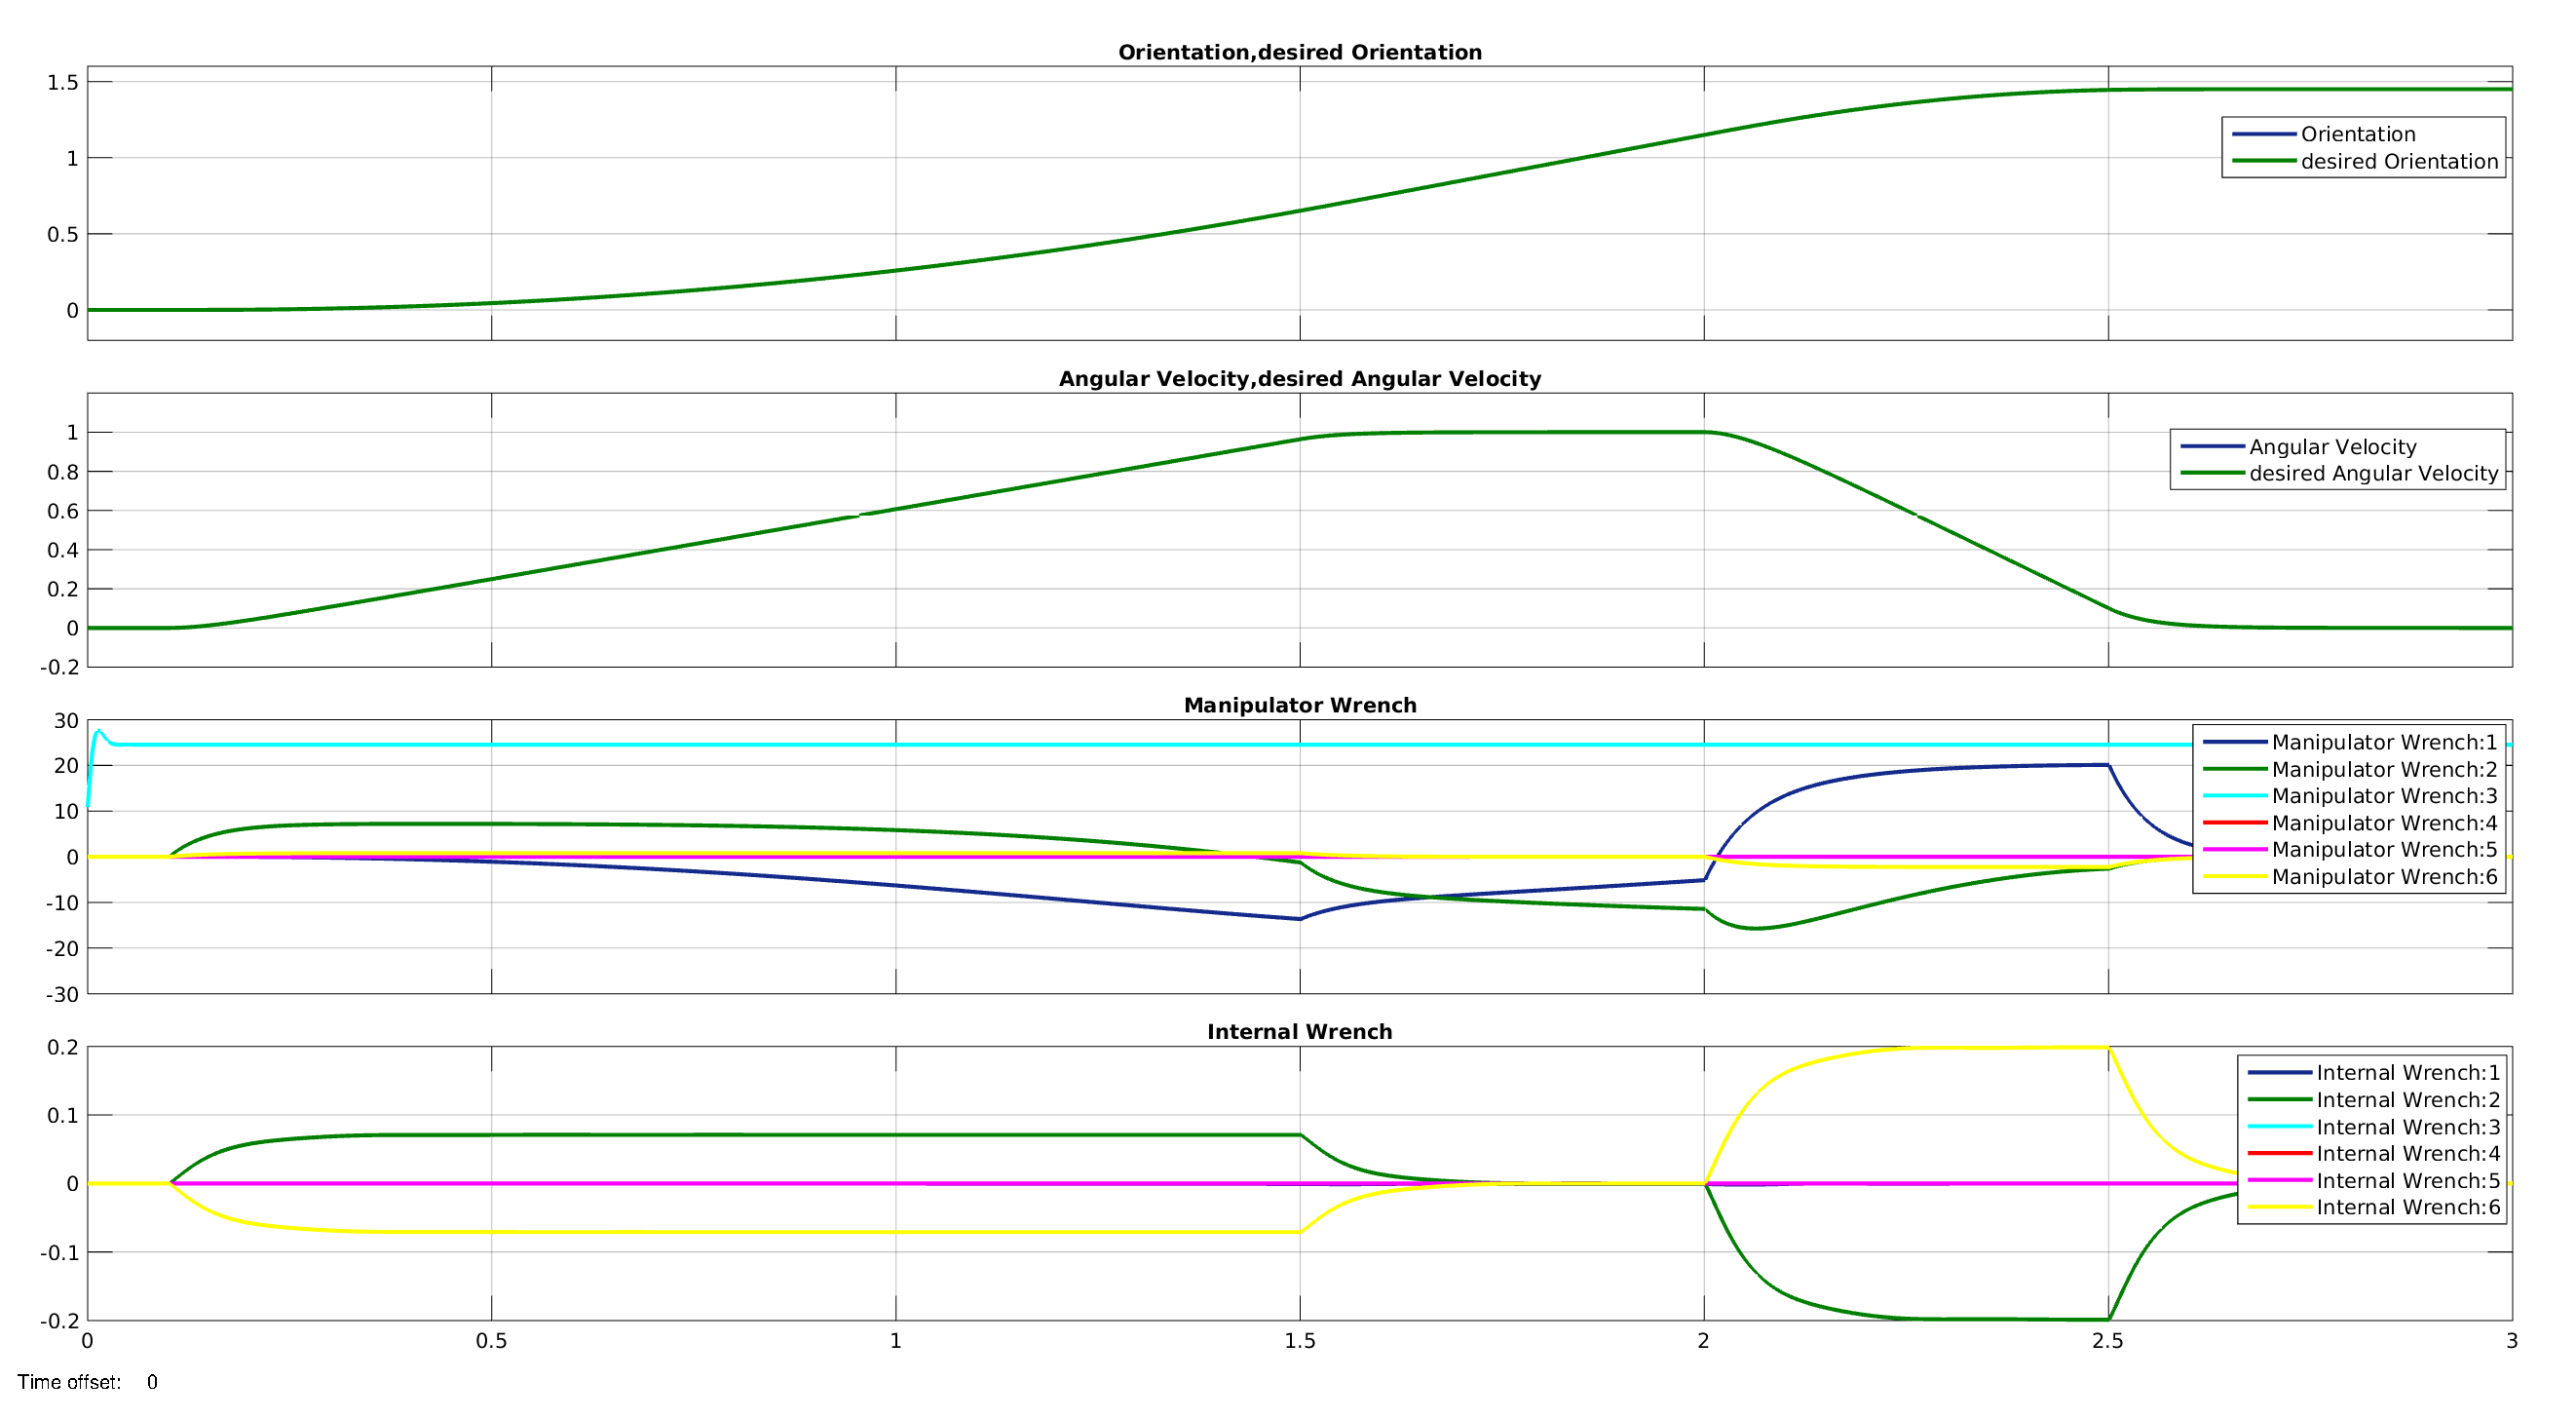
\includegraphics[width=0.9\textwidth]{Caccavaleorientation.eps}
			\caption{Position, Velocity, Manipulator wrench, Internal wrench}
\end{figure}
\end{frame}

\begin{frame}
	\frametitle{Comparison of Grasp Controllers 2}
Internal impedance control with object force-feedforward \cite{DePascali_15}
 \begin{figure}[htb]
			\centering
			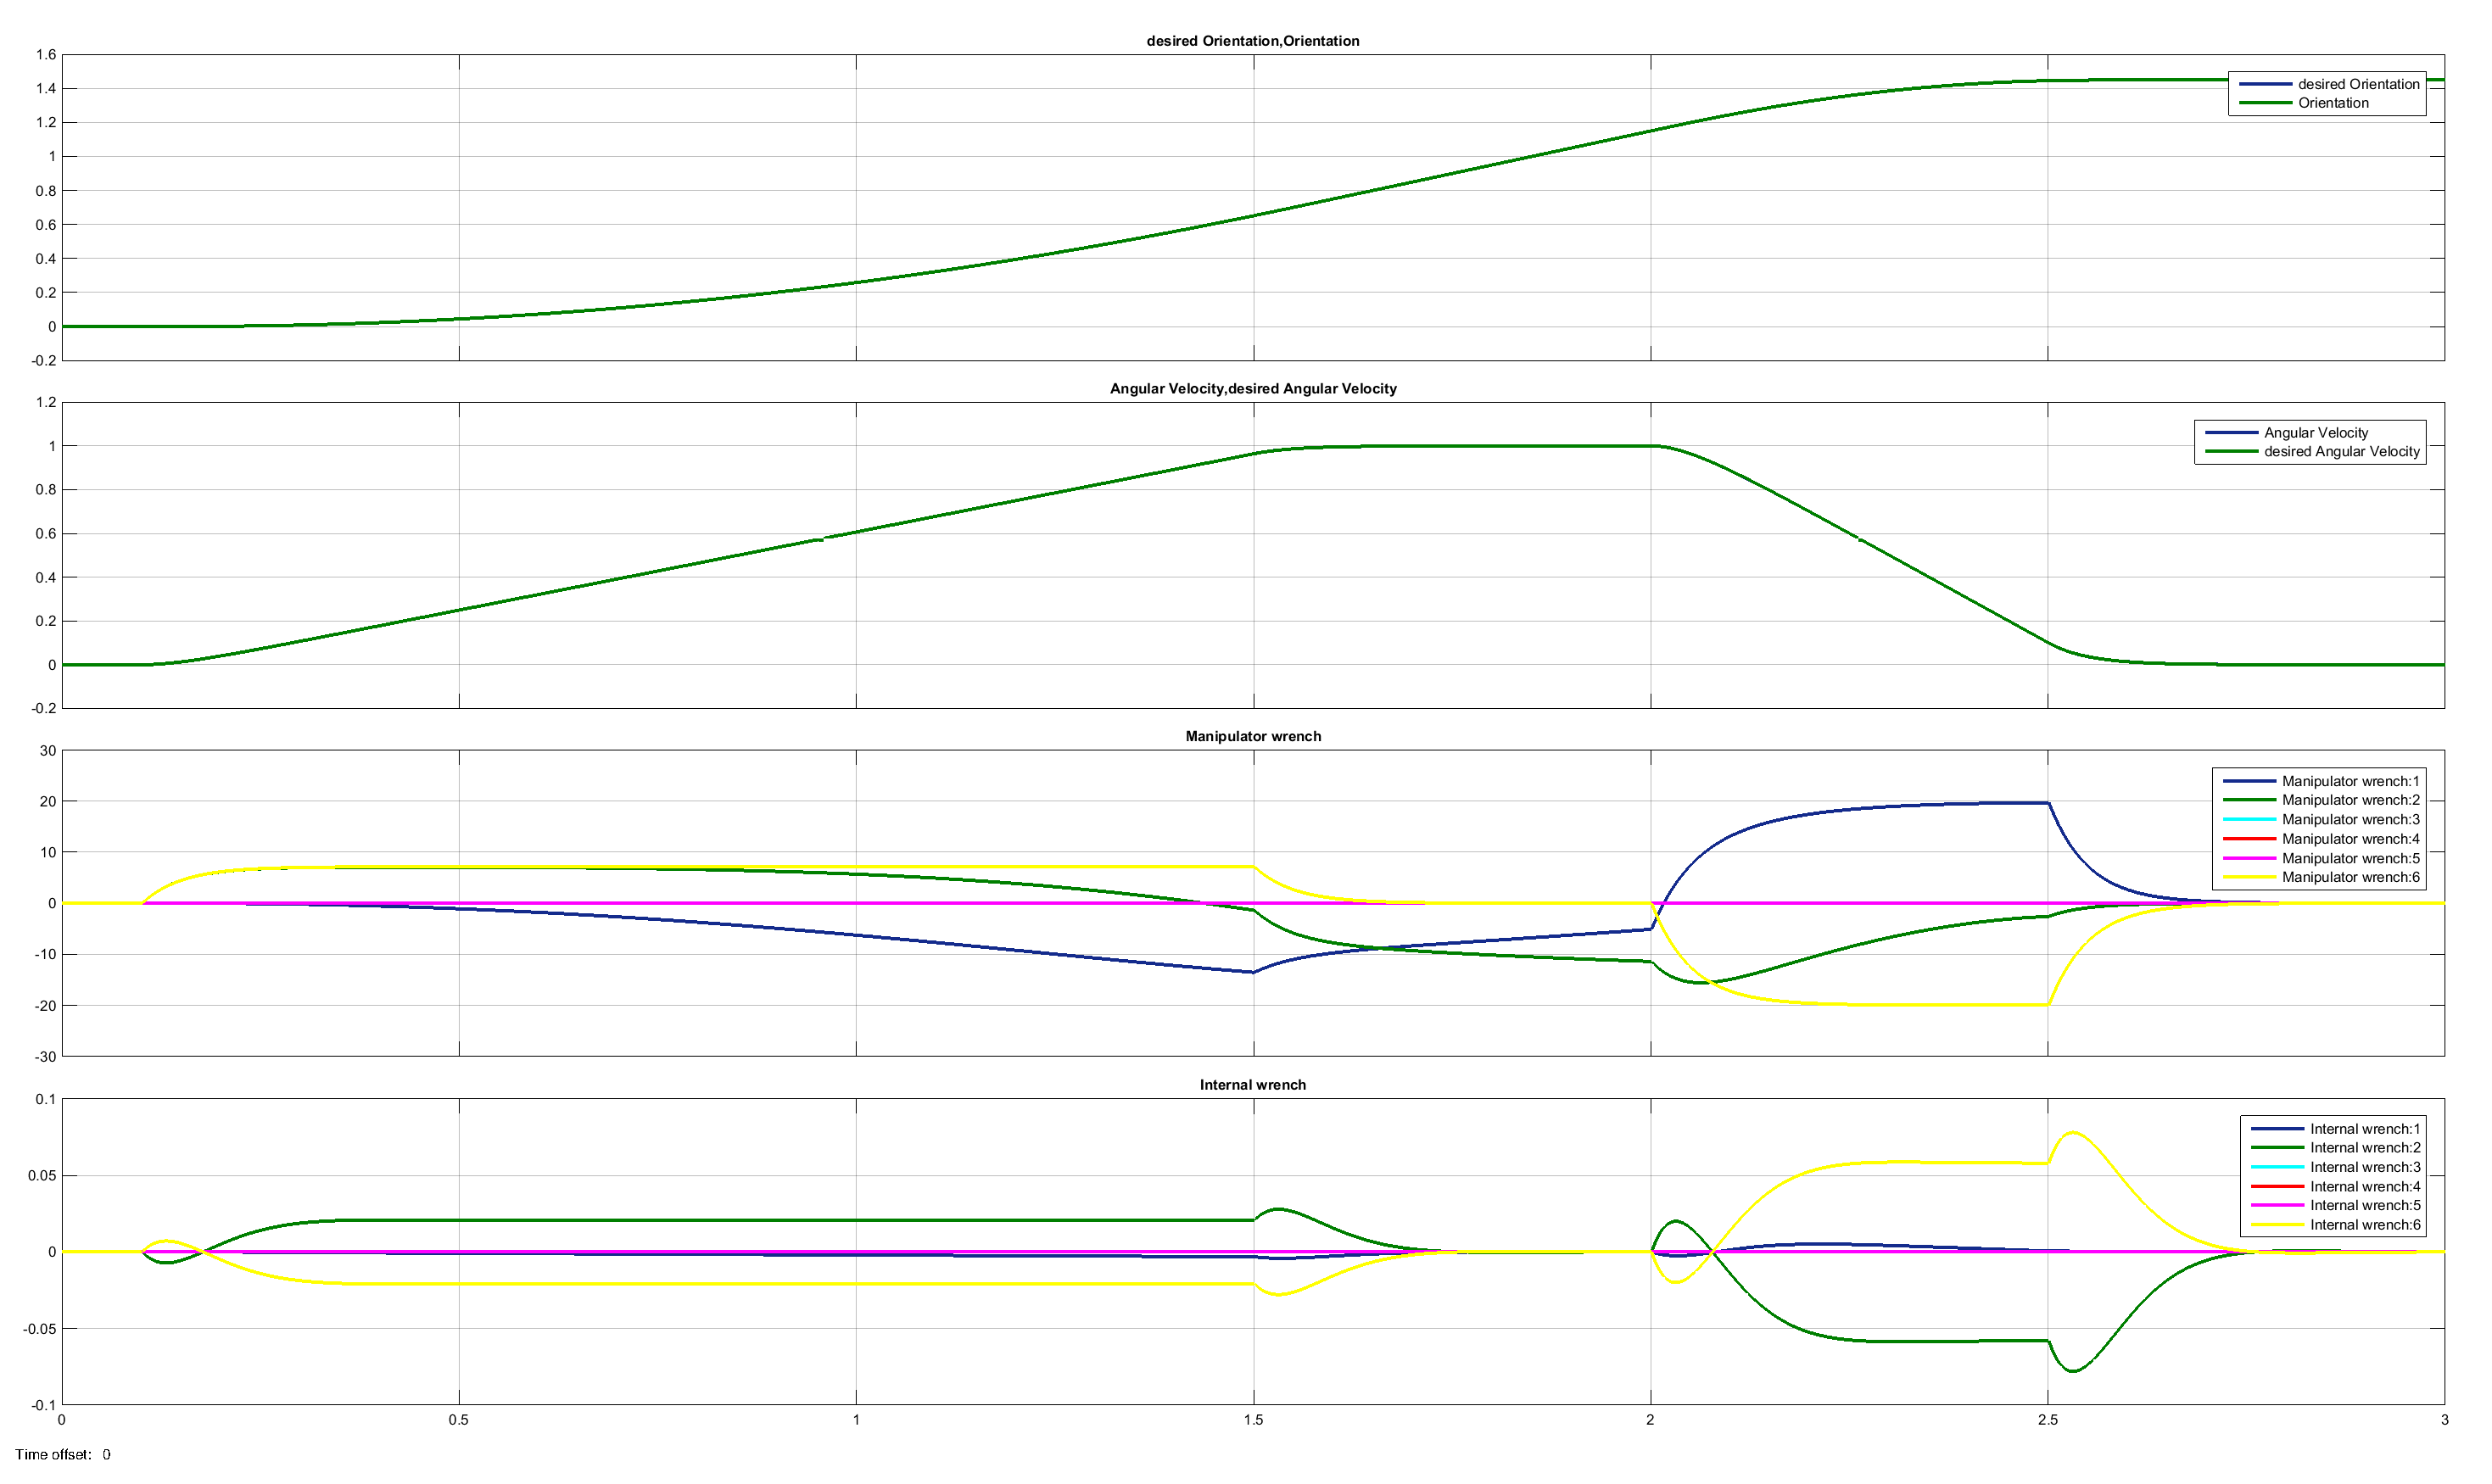
\includegraphics[width=0.9\textwidth]{Depascaliorientation.eps}
			\caption{Position, Velocity, Manipulator wrench, Internal wrench}
\end{figure}
\end{frame}

\section{Conclusion}

\begin{frame}
	\frametitle{Conclusion}
	...
\end{frame}
\appendix
%\nocite{buss11}
%\nocite{bauer09}
\begin{frame}
	\frametitle{References}
	%\tiny
	%\bibliographystyle{plain}
	%\bibliography{ref}
	\printbibliography
\end{frame}


\end{document}
